\section{Теоретические основы}

\subsection{Оценка временной сложности}

Временная сложность алгоритма описывается с помощью нотации «О-большое» (Big-O). Для
алгоритма, выполняющего $T(n)$ операций на входе размером $n$, запись
$T(n) = O(f(n))$ означает, что существуют константы $c > 0$ и $n_0 \geq 1$ такие, что:

\begin{equation}
    \label{eq:big-o}
    T(n) \leq c \cdot f(n) \quad \text{для всех} \quad n \geq n_0.
\end{equation}

Среднее число сравнений при быстрой сортировке массива из $n$ элементов описывается
рекуррентным соотношением~\cite{cormen2009algorithms}:

\begin{equation}
    \label{eq:quicksort-recurrence}
    C(n) = n - 1 + \frac{1}{n} \sum_{k=1}^{n} \bigl(C(k-1) + C(n-k)\bigr),
    \quad C(0) = C(1) = 0.
\end{equation}

Решение этой рекуррентности даёт асимптотику $C(n) \approx 2n\ln n$, что соответствует
$O(n \log n)$. Для сортировки слиянием рекуррентное соотношение имеет вид:

\begin{equation}
    \label{eq:mergesort-recurrence}
    T(n) = 2T\!\left(\frac{n}{2}\right) + \Theta(n), \quad T(1) = \Theta(1).
\end{equation}

По мастер-теореме~\cite{cormen2009algorithms} решение уравнения~\eqref{eq:mergesort-recurrence}
составляет $T(n) = \Theta(n \log n)$ при любом распределении входных данных.

\subsection{Сравнение алгоритмов}

На рисунке~\ref{fig:complexity} показано сравнение временных сложностей $O(n)$,
$O(n \log n)$ и $O(n^2)$. Хорошо видно, что алгоритмы с квадратичной сложностью
(например, сортировка пузырьком или сортировка вставками) значительно уступают при
росте $n$.

\begin{figure}[H]
    \centering
    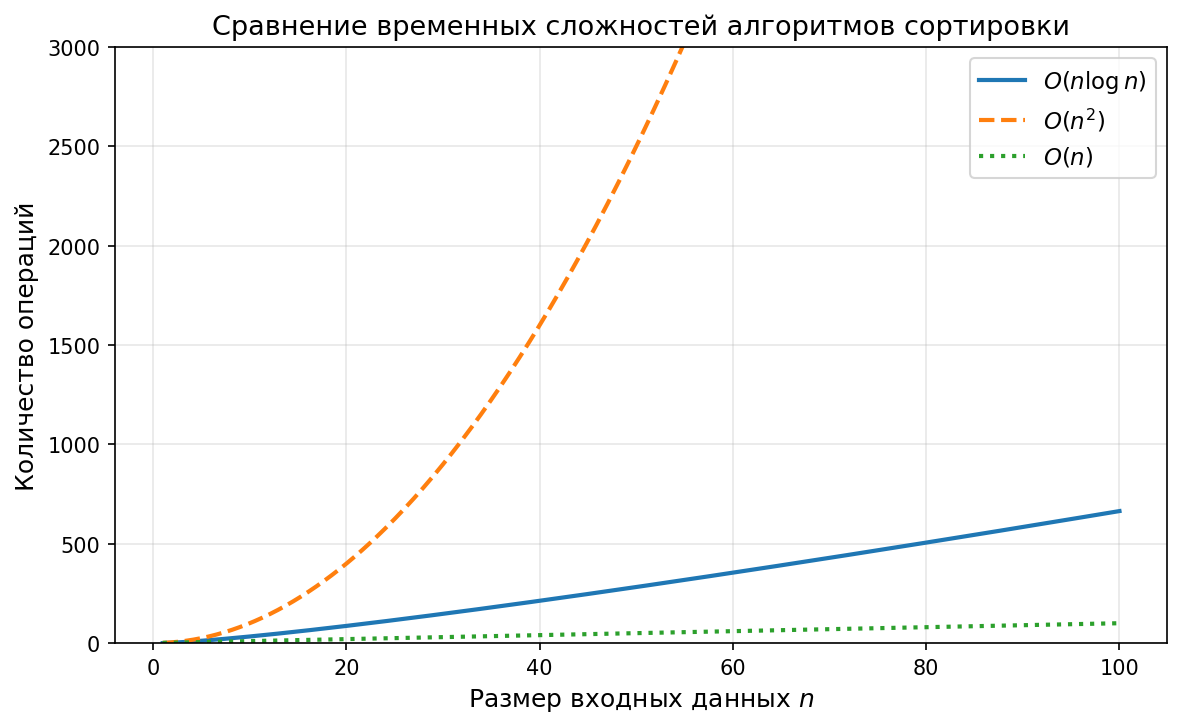
\includegraphics[width=0.82\textwidth]{img/complexity.png}
    \caption{Сравнение временных сложностей алгоритмов сортировки}
    \label{fig:complexity}
\end{figure}

В таблице~\ref{tab:comparison} приведено сравнение ключевых характеристик рассматриваемых
алгоритмов~\cite{sedgewick2011algorithms}.

\begin{table}[H]
    \centering
    \small
    \caption{Сравнение алгоритмов быстрой сортировки и сортировки слиянием}
    \label{tab:comparison}
    \begin{tabular}{lcccc}
        \toprule
        \textbf{Алгоритм} &
        \textbf{Лучший} &
        \textbf{Средний} &
        \textbf{Худший} &
        \textbf{Память} \\
        \midrule
        Быстрая сортировка   & $O(n \log n)$ & $O(n \log n)$ & $O(n^2)$      & $O(\log n)$ \\
        Сортировка слиянием  & $O(n \log n)$ & $O(n \log n)$ & $O(n \log n)$ & $O(n)$      \\
        Сортировка пузырьком & $O(n)$        & $O(n^2)$      & $O(n^2)$      & $O(1)$      \\
        Сортировка вставками & $O(n)$        & $O(n^2)$      & $O(n^2)$      & $O(1)$      \\
        \bottomrule
    \end{tabular}
\end{table}

\subsection{Принцип работы сортировки слиянием}

Сортировка слиянием рекурсивно разбивает массив пополам, сортирует каждую половину, а
затем сливает их в единый упорядоченный массив. На рисунке~\ref{fig:mergesort-steps}
проиллюстрированы основные этапы работы алгоритма для массива \texttt{[38, 27, 43, 3]}.

\begin{figure}[H]
    \centering
    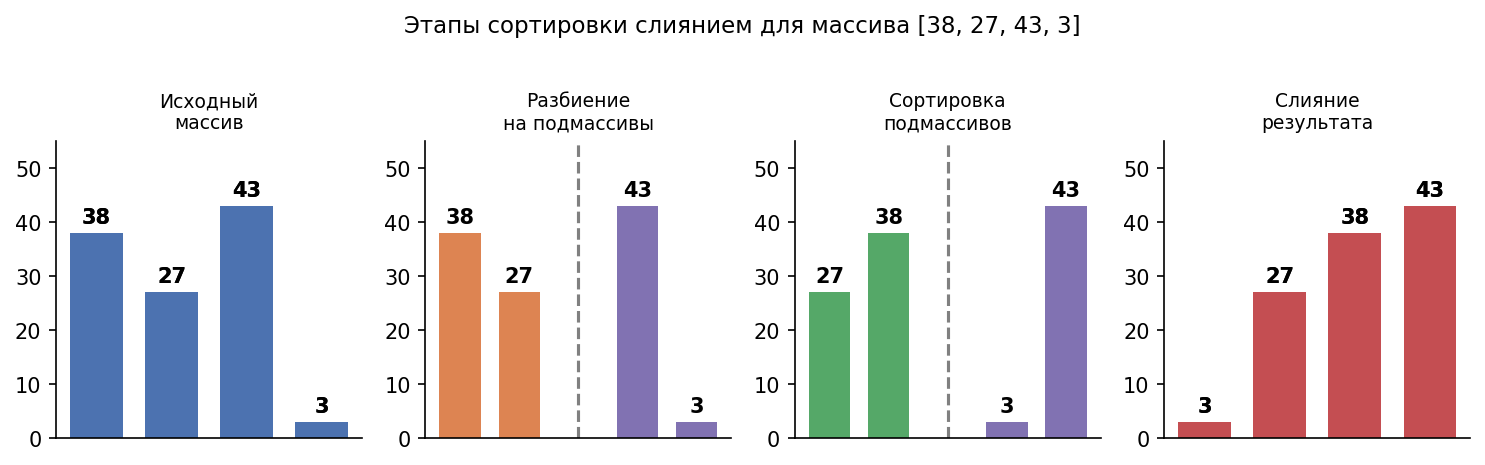
\includegraphics[width=0.90\textwidth]{img/mergesort_steps.png}
    \caption{Этапы выполнения сортировки слиянием}
    \label{fig:mergesort-steps}
\end{figure}
